\chapter{Retas}

\section{Equações da reta}

Uma reta $r$ pode ser representada por diferentes equações.

\subsection{Equação vetorial da reta}

Seja $A$ um ponto de uma reta $r$ que tem a direção de um vetor $v\neq 0$. Se um ponto $P$ pertence a $r$ então os vetores $\overrightarrow{AP}$ e $\vec v$ são colineares, isto é, existe um real $t$, tal que $\overrightarrow{AP}=t\vec v$ ou $P=A+t\vec v$.
\begin{multicols}{2}
\begin{figure}[H]
\centering
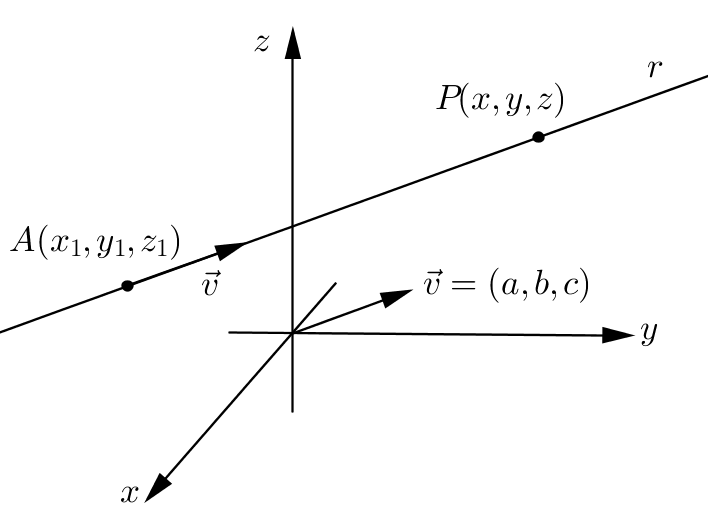
\includegraphics[scale=1]{analitica/imagens/reta-vetorial.png}
\end{figure}

$(x, y, z)=(x_1, y_1, z_1)+t(a,b,c)$

$\vec v$: vetor diretor da reta

$t$: parâmetro
\end{multicols}

\subsection{Equações paramétricas da reta}

Da equação vetorial da reta $r$, vem:

$$r:\left\{ \begin{array}{l}
x=x_1+at\\
y=y_1+bt\\
z=z_1+ct \end{array} \right. $$

\subsection{Equações simétricas da reta}

Admitindo-se $a$, $b$ e $c$ não nulos nas equações paramétricas e isolando o parâmetro $t$, vem:

$$\frac{x-x_1}{a}=\frac{y-y_1}{b}=\frac{z-z_1}{c}$$

\subsection{Equações reduzidas da reta}

Nas equações simétricas, escrevendo-se $y$ como função de $x$ e $z$ como função de $x$, vem:

$$r:\left\{ \begin{array}{l}
y=mx+n\\
z=px+q \end{array} \right. $$

\section{Retas paralelas aos eixos coordenados}

$r\parallel Ox \quad\Longleftrightarrow \quad \vec v \parallel \vec i \quad\Longleftrightarrow \quad r:\left\{ \begin{array}{l}
y=y_1\\
z=z_1 \end{array} \right.$

$r\parallel Oy \quad\Longleftrightarrow \quad \vec v \parallel \vec j \quad\Longleftrightarrow \quad r:\left\{ \begin{array}{l}
x=x_1\\
z=z_1 \end{array} \right.$

$r\parallel Oz \quad\Longleftrightarrow \quad \vec v \parallel \vec k \quad\Longleftrightarrow \quad r:\left\{ \begin{array}{l}
x=x_1\\
y=y_1 \end{array} \right.$


\textbf{Importante:}  Se duas componentes do vetor diretor forem nulas, a reta  é  paralela  ao  eixo  correspondente a componente não nula.

\section{Retas paralelas aos planos coordenados}

$r\parallel xOy \quad\Longleftrightarrow \quad \vec v \perp \vec k \quad\Longleftrightarrow \quad \vec v=(a,b,0) \quad\Longleftrightarrow \quad r:\left\{ \begin{array}{l}
x=x_1+at\\
y=y_1+bt\\
z=z_1 \end{array} \right.$

$r\parallel xOz \quad\Longleftrightarrow \quad \vec v \perp \vec j \quad\Longleftrightarrow \quad \vec v=(a,0,c) \quad\Longleftrightarrow \quad r:\left\{ \begin{array}{l}
x=x_1+at\\
y=y_1\\
z=z_1+ct \end{array} \right.$

$r\parallel yOz \quad\Longleftrightarrow \quad \vec v \perp \vec i \quad\Longleftrightarrow \quad \vec v=(0,b,c) \quad\Longleftrightarrow \quad r:\left\{ \begin{array}{l}
x=x_1\\
y=y_1+bt\\
z=z_1+ct \end{array} \right.$

\textbf{Importante:} Se uma das componentes do vetor diretor é nula, a reta é  paralela  ao  plano correspondente as componentes não nulas.

\section{Ângulo de duas retas}

O ângulo entre duas retas é o menor ângulo formado por dois vetores diretores das retas.

Se $\vec u$ e $\vec v$ são os vetores diretores das retas $r$ e $s$, então o ângulo entre as retas será dado por $\theta$, onde: $$\cos{\theta}=\frac{|\vec u \cdot \vec v|}{\Vert \vec u \Vert \Vert \vec v \Vert} \qquad 0\leq \theta \leq \frac{\pi}{2}$$

\subsection{Retas paralelas}

$r_1\parallel r_2 \quad\Longleftrightarrow \quad \vec v_1 \parallel \vec v_2$

\subsection{Retas ortogonais}

$r_1\perp r_2 \quad\Longleftrightarrow \quad \vec v_1 \perp \vec v_2$

\subsection{Reta ortogonal a duas retas}

Seja $r$ é uma reta ortogonal à duas retas não paralelas $r_1$ e $r_2$ com vetores diretores $\vec v_1$ e $\vec v_2$.

O vetor diretor de $r$ é qualquer vetor com a direção de $\vec v=\vec v_1 \times \vec v_2$.


\section{Intersecção de duas retas}

Sejam $r$ e $s$ duas retas concorrentes, então o ponto de intersecção $I$, é a solução do sistema formado pelas equações das retas $r$ e $s$.

\section{Retas coplanares}

Duas retas são coplanares se são paralelas ou concorrentes.

\textbf{Observação:} Duas retas não-coplanares são chamadas reversas

\textbf{Importante:} Retas perpendiculares são retas ortogonais e coplanares.